\chapter{Methodology}

\label{chapter:methodology}

% Camera calibration
% This is done by knowing the 3D position of each interest point and it's projections (colored sircles on \autoref{fig:calib}), and after taking a sample of images on a static camera and the pattern moving along X and Y axis with different scale and skew.
% Then some algorithm can be used to estimate unknown parameters of a calibration matrix, for example: estimate the camera projection matrix (can be done from 6 correspondences) and decompose it to $R$, $\vec{t}$ and $K$ 

% The problem solution can be divided into several steps. 
% Firstly, it is necessary to make a math model of a device that can solve the problem and describe its behaviour. 
% The next step is to make a CAD model of the cameras' holder, print and assemble it, and then calibrate it. 
% Then detect features and compute the distance to visible objects in cameras' overlapping zone: as far as a stereo pair is calibrated, the precision depends on a stereo pair calibration, cameras' calibration, key point extractor and matcher.
% As a result, provided points and features can be used in an SfM algorithm to correct a relative stereo pair position in time while moving and in a feedback loop inside the MRS system to correct its path planning concerning found obstacles.
The main task of this thesis is to create a compact obstacle avoidance system such that it can be mount on MAVs with size and weight restrictions.
There are related works of a monocular stereovision using SfM or Optical flow algorithms, also there are some stereovison approaches with a standard stereocameras as on \autoref{fig:stereo_ex}.

The method that combines monocamera and stereocamera approaches is presented further.

\section{Model description}

\begin{figure}[h]
    \centering
    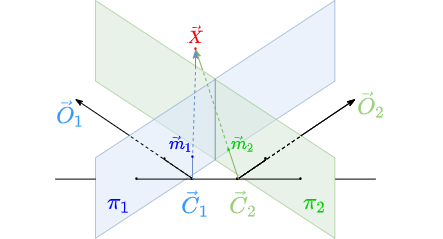
\includegraphics[width=.7\textwidth]{graphics/td90deg.png}
    \caption{The proposed approach model}
    \label{fig:td90deg}
\end{figure}

On the \autoref{fig:td90deg}: there are two cameras with centers at $C_1$ and $C_2$ with a known static translation $\vec{t}_{21}$ and rotation $\mat{R}_{21}$, where $\mat{R}_{21}$ corresponds to Euler angle $90^\circ$ rotation in the epipolar plane (\autoref{fig:epipolar_std}, plane $\sigma$).
Both cameras' intrinsic parameters are known and images are synchronized in time, FOV of both cameras have an interesting zone.
Let images from cameras with centers at $C_1$ and $C_2$ be \textit{im1} and \textit{im2} respectively.
In the overlapping zone, there are two interesting points detected and matched as images of a same 3D point $\vec{X}$: $\vec{m}_1$ on \textit{im1} and $\vec{m}_2$ on \textit{im2}.
The 3D pose of a point $\vec{X}$ in world measurement units is obtain from known vectors $\vec{X} - \vec{C}_1$, $\vec{X} - \vec{C}_2$ and $\vec{t_{21}}$. 

Described method assumes that each camera is calibrated, stereopair is also calibrated - both $t_{21}$ and $R_{21}$ are known.

\section{General multicamera calibration}
There are multiple algorithms to do a stereopair calibration (\autoref{sec:prelimin_stereocalib}). 
Usually calibration chessboard is used (\autoref{fig:calib}) for a standard stereocamera with paralell or converging optical rays.
It can be detected and used only when the whole chessboard is seen on both images.
For cameras with a small overlapping zone and diverging optical rays it is a disadvantage, only if a really big chessboard is used on a relatively big distance.
For this reason it is better to use some other pattern, for example set of apriltags \cite{Malyuta2019}. 

\subsection{Least-square estimation of transformation}
\label{sec:lsq_umeyama}
The first approach assumes that cameras poses are pre-known and the only necessary step is to correct one camera pose with respect to another.
Firstly it detects apriltag's from \textit{im1} and \textit{im2}, compute their 3D poses.
Then, estimate a transformation parameters between two point sets, which means find a corection transformation $T_{correction}$.
After it is done, 
apply it to correct $\mat{R}_{21}$ and $\vec{t}_{21}$.

\subsection{PnP-based}
Another, more general approach is based on a solving of a Perspective-n-Point (PnP) problem.
General PnP is the problem of estimation a camera pose given a known set of 3D points and it's 2D projections. 
For this algorith no initial pose estimation is needed, but if there is one - it can accelerate the solver.

% \subsection{}
% It is also possible to make a calibration having correctly matched correspondences only, but the pressision can be worse.
% Having two calibrated cameras, it is possible to compute essential matrix $\mat{E}$ \autoref{eq:E} from at least 5 corresponding points, and then decompose it to $\mat{R}_{21}$ and $\vec{t}_{21}$.

\section{Features extraction and matching}

\section{Features pose estimation}

